% =====================================================================
% IEEE WCNC 2027 submission draft (6 pages max, not blind, EDAS).
% Title and author list must match the EDAS registration exactly.
%
% NUMBERS: every quoted result is a macro. paper/numbers.tex (generated
% by scripts from results/, evaluation seeds) defines them with
% \newcommand; the \providecommand defaults below are the current values
% copied from the M1-M3 reports and are shown in BLUE until numbers.tex
% exists. Macro list (numbers.tex must define exactly these):
%   \numEventsPerMin \numBusShare \numPedShare \numSameCellLoss
%   \numOtherCellBus \numOtherCellPed \numOnsetBus \numOnsetPed
%   \numBusPd \numPedPd \numFA \numLeadBus \numLeadPed
%   \numMapBus \numMapPed \numMapCross \numGhostGain
%   \numRefMargin \numSNRreq \numOverhead
%   \numAthreeTen \numOracleTen \numGenieTen \numHybridTen \numXappTen
%   \numAthreeRef \numOracleRef \numGenieRef \numHybridRef
%   \numGenieMatch \numAthreeMatch \numGeniePreBus \numAthreePreBus
%   \numForesightRange \numForesightRef \numForesightMaxAbs
%   \numTauZeroLow \numTauZeroHigh \numTauZeroRef
% Definitions (evaluation seeds, M2 two-O-RU config, serving cell =
% strongest unblocked; ranges are min--max over mounts unless noted):
%   EventsPerMin: 10 dB serving-LoS events per UE-minute, pooled.
%   BusShare/PedShare: share of those events by dominant blocker class.
%   SameCellLoss: median best surviving same-cell path after model B,
%     relative to unblocked LoS [dB].
%   OtherCellBus/Ped: share of events with the other cell clear (<3 dB).
%   OnsetBus/Ped: median 10-90% rise time of 10 dB events [s].
%   BusPd/PedPd/FA: final M2 config, budget 4: track Pd, FA per CPI.
%   LeadBus/Ped: confirmed track 0.5 s before onset (final M2 config).
%   MapBus/MapPed/MapCross: unconstrained -> map tracker ("a to b").
%   GhostGain: bus/truck track Pd, no-ghost -> image at budget 4 ("a to b").
%   RefMargin, SNRreq [dB]; Overhead: sensing overhead.
%   *Ten / *Ref: outage [s/UE-min] at 10 dB margin / 3GPP reference.
%   GenieMatch/AthreeMatch: share of HOs matching a 10 dB event.
%   GeniePreBus/AthreePreBus: bus/truck events with HO before onset.
%   ForesightRange (min--max over 5-30 dB), ForesightRef: causal foresight
%     bound = blockage-caused wrong-cell time (A3's cell unusable, other
%     cell usable, A3's cell usable without blockers), pooled share of A3
%     outage over evaluation jobs; ForesightMaxAbs: max over margins
%     [s/UE-min].
%   TauZeroLow (0-10 dB), TauZeroHigh (15-30 dB), TauZeroRef: share of
%     the A3-oracle gap closed by tau_HO = 0.
% FIGURES: scripts write paper/figs/fig_onset.pdf, fig_leadtime.pdf,
% fig_outage_margin.pdf, fig_headroom.pdf; placeholders until they exist.
% RED = text still to be written or checked.
% =====================================================================
\documentclass[conference]{IEEEtran}
\IEEEoverridecommandlockouts
\usepackage{cite}
\usepackage{amsmath,amssymb,amsfonts}
\usepackage{graphicx}
\usepackage{booktabs}
\usepackage{siunitx}
\usepackage{xcolor}
\usepackage{tikz}
\usetikzlibrary{arrows.meta,patterns}
\usepackage[hidelinks]{hyperref}

\newcommand{\prelim}[1]{\textcolor{blue}{#1}}
\newcommand{\tbd}[1]{\textcolor{red}{[TBD: #1]}}

\IfFileExists{numbers.tex}{% Generated by scripts/make_paper.py from results/. Do not edit.
\newcommand{\numEventsPerMin}{8.5}
\newcommand{\numBusShare}{44--47\%}
\newcommand{\numPedShare}{53--56\%}
\newcommand{\numSameCellLoss}{26--34}
\newcommand{\numOtherCellBus}{68--71\%}
\newcommand{\numOtherCellPed}{27--34\%}
\newcommand{\numOnsetBus}{0.50}
\newcommand{\numOnsetPed}{0.01}
\newcommand{\numBusPd}{0.94}
\newcommand{\numPedPd}{0.46}
\newcommand{\numFA}{3.9}
\newcommand{\numLeadBus}{84--90\%}
\newcommand{\numLeadPed}{53--63\%}
\newcommand{\numMapBus}{0.82 to 0.90}
\newcommand{\numMapPed}{0.28 to 0.45}
\newcommand{\numMapCross}{2.0 to 0.5}
\newcommand{\numGhostGain}{0.82 to 0.88}
\newcommand{\numRefMargin}{35.9}
\newcommand{\numSNRreq}{9.3}
\newcommand{\numOverhead}{2.3\%}
\newcommand{\numAthreeTen}{3.43}
\newcommand{\numOracleTen}{2.87}
\newcommand{\numGenieTen}{3.48}
\newcommand{\numHybridTen}{5.32}
\newcommand{\numXappTen}{6.25}
\newcommand{\numAthreeRef}{0.20}
\newcommand{\numOracleRef}{0.02}
\newcommand{\numGenieRef}{0.23}
\newcommand{\numHybridRef}{0.33}
\newcommand{\numGenieMatch}{87\%}
\newcommand{\numAthreeMatch}{44\%}
\newcommand{\numGeniePreBus}{70\%}
\newcommand{\numAthreePreBus}{23\%}
\newcommand{\numForesightRange}{2--9\%}
\newcommand{\numForesightRef}{16\%}
\newcommand{\numForesightMaxAbs}{0.32}
\newcommand{\numTauZeroLow}{35--42\%}
\newcommand{\numTauZeroHigh}{68--93\%}
\newcommand{\numTauZeroRef}{97\%}
}{}
\providecommand{\numEventsPerMin}{\prelim{8.8}}
\providecommand{\numBusShare}{\prelim{59--75\%}}
\providecommand{\numPedShare}{\prelim{25--41\%}}
\providecommand{\numSameCellLoss}{\prelim{26--33}}
\providecommand{\numOtherCellBus}{\prelim{56--59\%}}
\providecommand{\numOtherCellPed}{\prelim{25--29\%}}
\providecommand{\numOnsetBus}{\prelim{0.5}}
\providecommand{\numOnsetPed}{\prelim{0.01}}
\providecommand{\numBusPd}{\prelim{0.94}}
\providecommand{\numPedPd}{\prelim{0.47}}
\providecommand{\numFA}{\prelim{3.9}}
\providecommand{\numLeadBus}{\prelim{84--90\%}}
\providecommand{\numLeadPed}{\prelim{53--63\%}}
\providecommand{\numMapBus}{\prelim{0.82 to 0.90}}
\providecommand{\numMapPed}{\prelim{0.28 to 0.45}}
\providecommand{\numMapCross}{\prelim{2.0 to 0.5}}
\providecommand{\numGhostGain}{\prelim{0.80 to 0.86}}
\providecommand{\numRefMargin}{\prelim{35.9}}
\providecommand{\numSNRreq}{\prelim{9.3}}
\providecommand{\numOverhead}{\prelim{2.3\%}}
\providecommand{\numAthreeTen}{\prelim{3.43}}
\providecommand{\numOracleTen}{\prelim{2.87}}
\providecommand{\numGenieTen}{\prelim{3.48}}
\providecommand{\numHybridTen}{\prelim{5.32}}
\providecommand{\numXappTen}{\prelim{6.25}}
\providecommand{\numAthreeRef}{\prelim{0.20}}
\providecommand{\numOracleRef}{\prelim{0.02}}
\providecommand{\numGenieRef}{\prelim{0.23}}
\providecommand{\numHybridRef}{\prelim{0.33}}
\providecommand{\numGenieMatch}{\prelim{87\%}}
\providecommand{\numAthreeMatch}{\prelim{44\%}}
\providecommand{\numGeniePreBus}{\prelim{70\%}}
\providecommand{\numAthreePreBus}{\prelim{23\%}}
\providecommand{\numForesightRange}{\prelim{1--8\%}}
\providecommand{\numForesightRef}{\prelim{15\%}}
\providecommand{\numForesightMaxAbs}{\prelim{0.19}}
\providecommand{\numTauZeroLow}{\prelim{35--42\%}}
\providecommand{\numTauZeroHigh}{\prelim{68--93\%}}
\providecommand{\numTauZeroRef}{\prelim{97\%}}

% figure helper: include the PDF if it exists, otherwise a placeholder
\newcommand{\figorbox}[3]{%
  \IfFileExists{figs/#1}{\includegraphics[width=\columnwidth]{figs/#1}}%
  {\fbox{\parbox[c][#2][c]{0.92\columnwidth}{\centering
   \textcolor{red}{Placeholder: \detokenize{figs/#1}. #3}}}}}

\begin{document}

\title{Revisiting ISAC-Enabled Proactive Handover for\\
Blockage-Resilient mmWave Open RAN}

\author{
\IEEEauthorblockN{Seyed Bagher Hashemi Natanzi\IEEEauthorrefmark{1}\textsuperscript{,}\thanks{*Corresponding author: snatanzi@wpi.edu}, Bo Tang\IEEEauthorrefmark{2}}
\IEEEauthorblockA{\IEEEauthorrefmark{1}\IEEEauthorrefmark{2}Department of Electrical and Computer Engineering, Worcester Polytechnic Institute (WPI), USA}
\IEEEauthorblockA{Email: \{snatanzi, btang1\}@wpi.edu}
}

\maketitle

\begin{abstract}
Integrated sensing and communication (ISAC) promises to let a
millimeter-wave (mmWave) network see blockers coming and hand users over
before the link breaks. We ask how much such foresight can actually gain
over standard reactive handover. Using a spatially consistent ray-traced
model of a \SI{28}{GHz} street canyon, in which the same 3GPP sensing
targets scatter radar echoes and obstruct communication paths, we build
a complete pipeline: monostatic OFDM radar at the radio unit,
digital-twin-aware tracking, blockage prediction, and a handover xApp
for the Open RAN near-real-time RIC. Sensing works: heavy vehicles,
which together with pedestrians cause all line-of-sight outages, are
tracked \SI{0.5}{s} before blockage onset in \numLeadBus{} of cases.
Yet neither the sensing-driven xApp nor a genie with perfect blockage
prediction outperforms 3GPP A3 handover at any link margin. A
policy-independent bound shows that foresight can recover at most
\numForesightRange{} of the reactive outage. Two physical facts explain
this: blockers that are predictable (buses, trucks) cause slow outages
that A3 already follows, whereas abrupt outages come from nearby
pedestrians who are hard to track and often shadow both cells. The
remaining gap is dominated by wrong-cell lag at low margins and by
handover interruption at high margins; interruption-free handover closes
up to \numTauZeroRef{} of it at the 3GPP reference margin.
\end{abstract}

\begin{IEEEkeywords}
ISAC, mmWave blockage, proactive handover, O-RAN, ray tracing, digital twin.
\end{IEEEkeywords}

% ---------------------------------------------------------------------
\section{Introduction}
% ---------------------------------------------------------------------
Millimeter-wave links lose tens of decibels when a body crosses the line
of sight (LoS) \cite{rappaport2013mmwave,maccartney2017blockage}. A
natural remedy is foresight: if the network knew that a bus is about to
cross a user's LoS, it could move the user to another cell in advance.
Prior work has predicted blockage and triggered proactive handoff from
cameras or dedicated radars \cite{charan2021vision,demirhan2022radar,alkhateeb2023deepsense}.
Integrated sensing and communication (ISAC) removes the extra sensors:
the radio unit senses with its own OFDM waveform
\cite{liu2022isac,sturm2011ofdm}, 3GPP has studied ISAC use cases and
standardized sensing-target channel models \cite{3gpp22837,3gpp38901},
and Open RAN (O-RAN) lets an xApp act on such information through the
E2 interface \cite{polese2023oran,bonati2021intelligence}.

The premise of this line of work is that foresight is valuable. We test
that premise directly by asking: \emph{how much of a user's outage can
any blockage prediction remove, relative to standard reactive
handover?} Answering this requires a model in which the blocker that the
radar sees is the same object that attenuates the link, a realistic
sensing pipeline, a fairly tuned reactive baseline, and an upper bound
that does not depend on the quality of a particular predictor.

Our contributions are:
\begin{itemize}
\item A spatially consistent ISAC--blockage simulation built on
Sionna~RT~2.2 \cite{hoydis2023sionnart}: every moving body is a
3GPP TR~38.901 radar target and, through blockage model~B, an obstacle
for communication paths. The pipeline is deterministic (bitwise
reproducible) and released as open source \tbd{repository link}.
\item A characterization of which blockers matter: passenger cars never
obstruct the LoS of \SI{5}{m}--\SI{8}{m} radio units, a blocker shadows
every path of the serving cell, and outages from heavy vehicles rise an
order of magnitude more slowly than those from pedestrians.
\item A sensing pipeline with digital-twin-aware ghost handling and
map-constrained tracking that detects most heavy blockers well before
onset.
\item An evaluation across link margins against tuned A3 handover,
including a genie predictor and a policy-independent foresight bound,
showing that foresight yields no significant gain and identifying
handover interruption and wrong-cell lag as the actual limits.
\end{itemize}

% ---------------------------------------------------------------------
\section{System Model}
% ---------------------------------------------------------------------
\subsection{Deployment, Targets, and Mobility}
We model an \SI{80}{m} street canyon (periodic, constant traffic
density) at $f_c=\SI{28}{GHz}$ with two radio units (O-RUs) that form two
cells. O-RU~0 is on the north side, on a lamppost (\SI{5}{m}) or a
facade (\SI{8}{m}); O-RU~1 is a \SI{5}{m} lamppost on the south sidewalk,
half a block away. Each O-RU has an $8\times8$ half-wavelength array;
pedestrian user equipments (UEs) carry one antenna at \SI{1.5}{m} on the
south sidewalk. Traffic consists of cars ($5\times2\times\SI{1.6}{m}$),
buses ($12\times2.5\times\SI{3.2}{m}$), trucks ($8\times2.5\times\SI{3.5}{m}$),
and pedestrians who walk the sidewalks or cross the street. Every moving
body is a TR~38.901 sensing target \cite{3gpp38901} (five scattering
points for vehicles, one for pedestrians). Positions and speeds come
from random seeds; disjoint tuning and evaluation seed sets are used
throughout, and results are reported with 95\% confidence intervals over
ten evaluation seeds.

\subsection{Radar Channel and Processing}
O-RU~0 operates as a monostatic radar under an ideal full-duplex
assumption, transmitting on one element and receiving on its
$8\times8$ array. Sionna's RCS solver traces paths through the
scattering points, and the static background is traced separately. One
sensing OFDM symbol per slot (numerology~3, \SI{120}{kHz} spacing, 1024
subcarriers) gives a pulse repetition frequency of \SI{8}{kHz}, so a
coherent processing interval (CPI) of 256 slots ($\SI{32}{ms}$) yields
\begin{equation}
\Delta R=\frac{c}{2B}\approx\SI{1.2}{m},\qquad
\Delta v=\frac{\lambda}{2MT_s}\approx\SI{0.17}{m/s},
\label{eq:res}
\end{equation}
and an unambiguous velocity $v_{\max}=\lambda f_{\mathrm{PRF}}/4\approx\SI{21}{m/s}$.
One CPI is processed every \SI{0.1}{s}, so sensing occupies
\numOverhead{} of the resources. The processing chain comprises
range--Doppler--angle maps with thermal noise, two-dimensional
cell-averaging CFAR, image-method ghost rejection that uses the known
building walls of the digital twin, DBSCAN clustering, and an extended
Kalman filter on range, angles, and radial velocity. The map-constrained
variant restricts vehicles to lane center lines and pedestrians to
sidewalks, switching to a free model for crossings.

\subsection{Communication Channel and Blockage}
Ray-traced targets are perfect absorbers, which would make every
blockage infinitely deep. We therefore trace the communication paths
without targets and attenuate every segment of every path with 3GPP
blockage model~B \cite{3gpp38901}, which treats blocker $k$ as a screen
with loss
\begin{equation}
L_k=-20\log_{10}\!\bigl(1-(F_{h_1}+F_{h_2})(F_{w_1}+F_{w_2})\bigr),
\label{eq:modelB}
\end{equation}
where each knife-edge term is
$F=\pi^{-1}\arctan\!\bigl(\pm\frac{\pi}{2}\sqrt{\pi\lambda^{-1}(D_1+D_2-r)}\bigr)$
and $D_1$, $D_2$, $r$ are the edge and direct distances of the segment.
Losses add in decibels over blockers and segments, and are evaluated
every \SI{10}{ms} from the blockers' actual positions.

\subsection{Link Budget and Margin}
Transmit power (\SI{33}{dBm}) and UE noise figure (\SI{13}{dB}) follow
the dense-urban micro assumptions of TR~38.802 \cite{3gpp38802}; cable,
body, and implementation losses are left unspecified by 3GPP
\cite{3gpp38830} and set to \SI{0}{dB}. Each O-RU serves with its best
beam, and throughput is Shannon's rate capped at the highest NR
spectral efficiency \cite{3gpp38214}. A user is in outage when its SNR
is below $\mathrm{SNR}_{\mathrm{req}}=\numSNRreq$\,dB, the value needed
for \SI{400}{Mbit/s}; handover interruption counts as outage. We define
the link margin as the median unblocked best-cell SNR minus
$\mathrm{SNR}_{\mathrm{req}}$. With the 3GPP budget the margin is
\numRefMargin\,dB, too high for a typical \SI{20}{dB} blockage to cause
outage on these short links. Longer links, the losses left unspecified
by 3GPP, or higher rates lower it, so we sweep a common extra path loss
that sets the margin from 0 to \SI{30}{dB}.

\subsection{Handover Schemes}
All schemes are tuned separately at every margin on the tuning seeds.
\emph{A3} hands over when the neighbor's filtered RSRP exceeds the
serving one by an offset plus hysteresis for a time-to-trigger
\cite{3gpp38331}. \emph{RSRP-trend} adds a handover when the serving
RSRP is extrapolated to drop. The \emph{xApp} runs on top of A3: every
\SI{0.1}{s} it receives tracks over E2, predicts the LoS blockage of
both cells over a horizon $H$ from the tracks and the UE positions
(known with \SI{1}{m} error), and hands over in advance when the
serving cell is predicted to block and the other is predicted clear,
after an E2 loop delay of \SI{20}{ms}. The \emph{hybrid} tunes A3 and
the xApp jointly. The \emph{genie} replaces the prediction by the true
future blockage of both cells, and the \emph{onset-advance genie} only
advances handovers before onset while A3 stays active. The \emph{oracle}
selects the better cell every \SI{10}{ms} without delay or
interruption. Each handover interrupts the user plane for
$\tau_{\mathrm{HO}}=\SI{20}{ms}$.

% ---------------------------------------------------------------------
\section{Which Blockers Matter}
% ---------------------------------------------------------------------
Users experience about \numEventsPerMin{} LoS outage events
(\SI{10}{dB} model-B loss) per minute. Table~\ref{tab:classes}
summarizes the blocker classes; Fig.~\ref{fig:geometry} explains the
first row. For a UE at height $h_u$ and an O-RU at height $h_o$ and
horizontal distance $d$, the LoS height at horizontal distance $x$ from
the UE is $z(x)=h_u+(h_o-h_u)x/d$, i.e., \SI{2.7}{m}--\SI{3.3}{m} over
the near lane: above a car, but through a bus or truck. Pedestrians
block only near the UE end of the ray.

\begin{table}[t]
\centering
\caption{Blocker classes (10 dB LoS outages, both mounts).}
\label{tab:classes}
\setlength{\tabcolsep}{2.6pt}
\begin{tabular}{@{}lccccc@{}}
\toprule
Class & Share of & 10--90\% & Other cell & Track before \\
      & outages  & onset [s] & clear & onset (0.5 s) \\
\midrule
Bus/truck  & \numBusShare & \numOnsetBus & \numOtherCellBus & \numLeadBus\\
Pedestrian & \numPedShare & \numOnsetPed & \numOtherCellPed & \numLeadPed\\
Car        & 0\%          & --           & --               & --\\
\bottomrule
\end{tabular}
\end{table}

\begin{figure}[t]
\centering
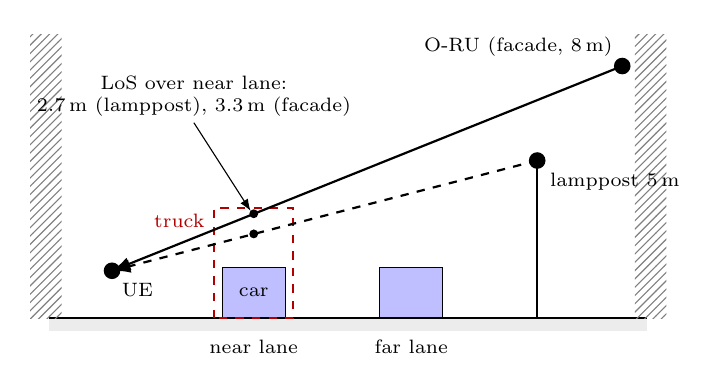
\begin{tikzpicture}[x=0.40cm,y=0.40cm,font=\scriptsize]
  \fill[gray!15] (-9,0) rectangle (10,-0.4);
  \draw[thick] (-9,0) -- (10,0);
  \fill[pattern=north east lines,pattern color=gray] (-9.6,0) rectangle (-8.6,9);
  \fill[pattern=north east lines,pattern color=gray] (9.6,0) rectangle (10.6,9);
  \node[below] at (-2.5,-0.4) {near lane};
  \node[below] at (2.5,-0.4) {far lane};
  \draw[fill=blue!25] (-3.5,0) rectangle (-1.5,1.6);
  \draw[dashed,red!70!black,thick] (-3.75,0) rectangle (-1.25,3.5);
  \node[red!70!black,left] at (-3.75,3.1) {truck};
  \node at (-2.5,0.8) {car};
  \draw[fill=blue!25] (1.5,0) rectangle (3.5,1.6);
  \fill (-7,1.5) circle (3pt); \node[below right] at (-7,1.4) {UE};
  \fill[black] (9.2,8) circle (3pt); \node[above left] at (9.2,8) {O-RU (facade, \SI{8}{m})};
  \draw[thick] (6.5,0) -- (6.5,5); \fill (6.5,5) circle (3pt);
  \node[below right] at (6.6,4.9) {lamppost \SI{5}{m}};
  \draw[thick,-{Latex}] (9.2,8) -- (-7,1.5);
  \draw[thick,dashed,-{Latex}] (6.5,5) -- (-7,1.5);
  \fill (-2.5,3.31) circle (1.6pt); \fill (-2.5,2.67) circle (1.6pt);
  \draw[-{Latex[length=1.5mm]},thin] (-4.4,6.2) -- (-2.6,3.4);
  \node[above,align=center] at (-4.4,6.1) {LoS over near lane:\\ \SI{2.7}{m} (lamppost), \SI{3.3}{m} (facade)};
\end{tikzpicture}
\caption{Street cross-section. Over the near lane the LoS passes above
cars but through tall vehicles.}
\label{fig:geometry}
\end{figure}

Two further observations shape the remedy. First, the blocker shadows
the whole angular sector of the serving O-RU, including the ground
reflection: the best surviving path lies a median \numSameCellLoss\,dB
below the unblocked LoS, so same-cell beam switching cannot recover the
link and only a second cell can. That cell is clear in most
heavy-vehicle outages but in few pedestrian outages, because a pedestrian
close to the UE shadows both cells. Second, the outages differ sharply in
dynamics (Fig.~\ref{fig:onset}): the loss caused by a bus or truck
rises over \numOnsetBus\,s, whereas a pedestrian next to the UE cuts
the link within \numOnsetPed\,s. A vehicle moving along the street
sweeps across the obliquely crossing LoS slowly, while a pedestrian
near the UE end of the ray covers it almost at once.
\tbd{verify this explanation with the onset figure.}

\begin{figure}[t]
\centering
\figorbox{fig_onset.pdf}{3.2cm}{Model-B loss vs.\ time for a median
bus/truck and pedestrian event; A3 and genie handover times marked.}
\caption{Blockage onset of a typical bus/truck and pedestrian event,
with the handover instants of A3 and the genie.}
\label{fig:onset}
\end{figure}

% ---------------------------------------------------------------------
\section{Sensing Performance}
% ---------------------------------------------------------------------
With the detector tuned on the tuning seeds to about \numFA{} false
alarms per CPI, the track detection probability is \numBusPd{} for buses
and trucks and \numPedPd{} for pedestrians, and a confirmed track exists
\SI{0.5}{s} before onset in \numLeadBus{} of heavy-vehicle and
\numLeadPed{} of pedestrian outages (Table~\ref{tab:classes}). We tested
three uses of the digital twin; the third was added after the first
results. Twin-based static-clutter subtraction is equivalent to blind
zero-Doppler removal, because static clutter has exactly zero Doppler in
simulation. Image-method ghost rejection does not raise detection at
identical parameters but removes 14--21\% of the unmatched clusters, so
at a fixed false-alarm budget it raises heavy-vehicle detection from
\numGhostGain{}. Map-constrained tracking raises detection from
\numMapBus{} (heavy vehicles) and \numMapPed{} (pedestrians), and reduces
the cross-lane velocity error from \numMapCross\,m/s
(Fig.~\ref{fig:leadtime}). Sensing therefore provides foresight for the
blockers that matter most.

\begin{figure}[t]
\centering
\figorbox{fig_leadtime.pdf}{3.2cm}{Share of 10 dB events with a
confirmed track before onset, map-constrained vs.\ unconstrained tracker.}
\caption{Share of outage events whose blocker is tracked a given time
before onset, per class, for the map-constrained and the unconstrained
tracker (95\% CI).}
\label{fig:leadtime}
\end{figure}

% ---------------------------------------------------------------------
\section{Does Foresight Help?}
% ---------------------------------------------------------------------
Fig.~\ref{fig:outage} shows the outage time per UE-minute versus link
margin. At \SI{10}{dB} margin, A3 reaches \numAthreeTen{} and the oracle
\numOracleTen{}~s/UE-min; the sensing xApp (\numXappTen) and the hybrid
(\numHybridTen) are worse than A3, and where their confidence
intervals separate from A3's they are always worse. RSRP-trend
prediction overlaps A3 at every margin. A Pareto comparison of outage
against handover rate and ping-pong rate shows that the hybrid dominates
no point of A3's front.

\begin{figure}[t]
\centering
\figorbox{fig_outage_margin.pdf}{3.6cm}{Outage [s/UE-min] vs.\ link
margin for A3, hybrid, genie + A3, oracle (95\% CI); 3GPP reference
margin marked.}
\caption{Outage time versus link margin for A3, the hybrid, the genie
(without sensing overhead) and the oracle (95\% CI). Neither the hybrid
nor the genie improves on A3.}
\label{fig:outage}
\end{figure}

The xApp's predictions are imperfect, so we remove that factor. The
genie, fed the true future blockage of both cells, triggers accurate
handovers (\numGenieMatch{} match a real outage, versus
\numAthreeMatch{} for A3) and moves users before onset in
\numGeniePreBus{} of heavy-vehicle outages (A3: \numAthreePreBus).
Still, it overlaps A3 at every margin (\numGenieTen{} vs.\
\numAthreeTen{} at \SI{10}{dB}; \numGenieRef{} vs.\ \numAthreeRef{} at
the reference margin), and so does the onset-advance genie.

To rule out a weak policy, Fig.~\ref{fig:headroom} decomposes A3's
outage by cause, using the unblocked channel as a counterfactual. The
part any foresight could recover is blockage-caused wrong-cell time: the
user's cell is unusable, the other cell is usable, and the user's cell
would have been usable without blockers. The parts foresight cannot
recover are handover interruption, intervals in which both cells are
unusable, and wrong-cell time that persists without blockers, which is
driven by distance. Foresight can recover at most \numForesightRange{}
of A3's outage between 5 and \SI{30}{dB} margin (at most
\numForesightMaxAbs~s/UE-min), and \numForesightRef{} of a very small
outage at the reference margin. The reason is the physics of
Section~III: the outages that sensing predicts well rise slowly enough
for A3 to follow, while the abrupt ones are pedestrian outages that are
harder to track and often leave no clear cell.

\begin{figure}[t]
\centering
\figorbox{fig_headroom.pdf}{3.6cm}{Stacked shares of A3 outage vs.\
margin: blockage-caused wrong cell, distance-caused wrong cell, handover
interruption, both cells unusable; plus A3 with $\tau_{\mathrm{HO}}=0$.}
\caption{Causal decomposition of A3's outage versus margin. Only the
blockage-caused wrong-cell band can be reduced by blockage prediction;
the curve shows A3 with interruption-free handover.}
\label{fig:headroom}
\end{figure}

What does limit A3? At low margins, its residual gap to the oracle is
dominated by wrong-cell lag around blockage onsets and distance-driven
cell changes; from \SI{15}{dB} upward, by handover interruption.
Repeating the evaluation with interruption-free handover
($\tau_{\mathrm{HO}}=0$, as approached by make-before-break mechanisms
such as dual active protocol stack handover \cite{3gpp38300}) closes
\numTauZeroLow{} of the A3--oracle gap at 0--\SI{10}{dB},
\numTauZeroHigh{} at 15--\SI{30}{dB}, and \numTauZeroRef{} at the
reference margin, while the genie stays level with A3.

% ---------------------------------------------------------------------
\section{Discussion and Limitations}
% ---------------------------------------------------------------------
Our results do not show that sensing is useless for mobility; they show
that, in this geometry, reactive handover already captures nearly all
of the gain that foresight could offer. Foresight would matter more
where predictable blockers cause abrupt outages, for example vehicles
crossing the LoS perpendicularly at intersections, where reactive
mobility must be slow for stability, or where more cells reduce the
share of unrecoverable intervals. The study has limitations: a single
street canyon, monostatic sensing with ideal full duplex, the
knife-edge model~B instead of full-wave diffraction, Shannon-based rates,
and UE positions known to the network. \tbd{check against final M5
results; trim to fit 6 pages.}

% ---------------------------------------------------------------------
\section{Conclusion}
% ---------------------------------------------------------------------
We tested whether ISAC-based foresight can improve handover against
mmWave blockage in Open RAN. Although the network detects most heavy
blockers well before they cut the link, neither a sensing-driven xApp
nor a perfect predictor outperforms 3GPP A3 handover. Blockers that are
predictable cause slow outages that reactive handover already follows,
and the remaining loss is due to handover interruption and to intervals
without a usable cell. For mmWave mobility, reducing interruption and
adding cell diversity therefore appear more effective than adding
foresight.

\section*{Acknowledgment}
This material is based upon work supported in part by NSF under Awards
CNS-2120442 and IIS-2325863, and NTIA under Award No.\ 51-60-IF007. Any
opinions, findings, and conclusions or recommendations expressed in this
publication are those of the author(s) and do not necessarily reflect
the views of the NSF and NTIA.

\bibliographystyle{IEEEtran}
\bibliography{refs}

\end{document}
